\documentclass[11pt]{article}
\usepackage[letterpaper,margin=1in]{geometry}
\usepackage[T1]{fontenc}
\usepackage[utf8]{inputenc}
\usepackage{lmodern}
\usepackage{microtype}
\usepackage{graphicx}
\usepackage{booktabs}
\usepackage{enumitem}
\usepackage{hyperref}
\usepackage{fancyhdr}
\usepackage{titlesec}
\usepackage{setspace}
\usepackage{caption}
\hypersetup{colorlinks=false,pdfborder={0 0 0}}
\setstretch{1.05}
\setlength{\headheight}{14pt}
\setlist[itemize]{leftmargin=1.4em}
\setlist[enumerate]{leftmargin=1.6em}
\providecommand{\tightlist}{}
\pagestyle{fancy}
\fancyhf{}
\fancyhead[L]{Localized Matched-Subspace Detection in Ultrasound Doppler Imaging}
\fancyhead[R]{Specification}
\fancyfoot[C]{\thepage}
\titleformat{\section}{\large\bfseries}{\thesection.}{0.5em}{}
\titleformat{\subsection}{\normalsize\bfseries}{\thesubsection.}{0.5em}{}

\begin{document}

\pagenumbering{gobble}

\begin{titlepage}
\centering
{\Large Systems and Methods for Localized Matched-Subspace Detection in Ultrasound Doppler Imaging\par}
\vspace{1.5cm}
{\large Specification\par}
\vspace{0.8cm}
\rule{0.72\textwidth}{0.6pt}\par
\vspace{0.8cm}
{\large U.S. Provisional Patent Application Specification and Drawings\par}
\vfill
{\large \today\par}
\end{titlepage}

\clearpage
\pagenumbering{arabic}
\setcounter{page}{1}

\tableofcontents
\clearpage

\input{generated/provisional_spec_body.tex}

\appendix
\clearpage
\section*{Drawings Appendix}
\addcontentsline{toc}{section}{Drawings Appendix}

\begin{figure}[p]
\centering
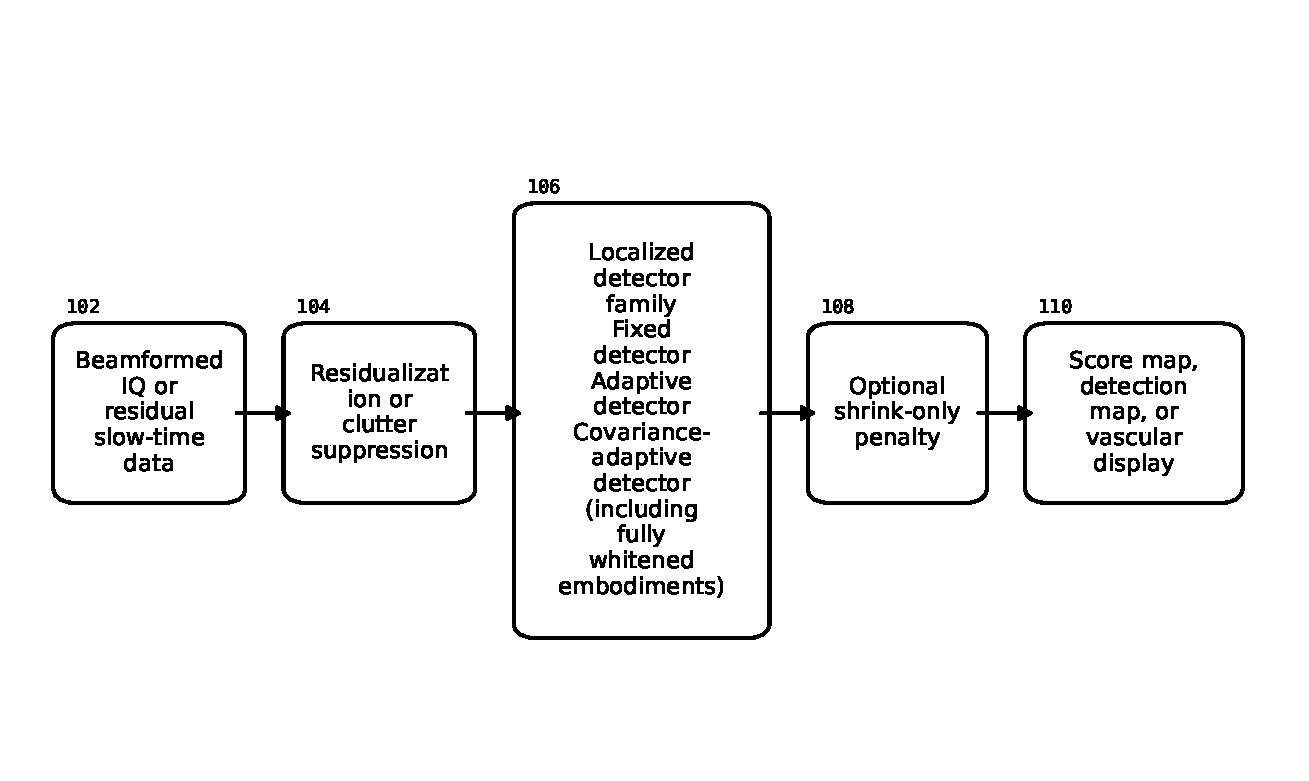
\includegraphics[width=\textwidth,height=0.72\textheight,keepaspectratio]{figs/figure_01_overview.pdf}
\caption*{Figure 1. End-to-end processing overview showing beamformed input data, residualization, localized detector branches, optional shrink-only penalty, and output score generation.}
\end{figure}
\clearpage

\begin{figure}[p]
\centering
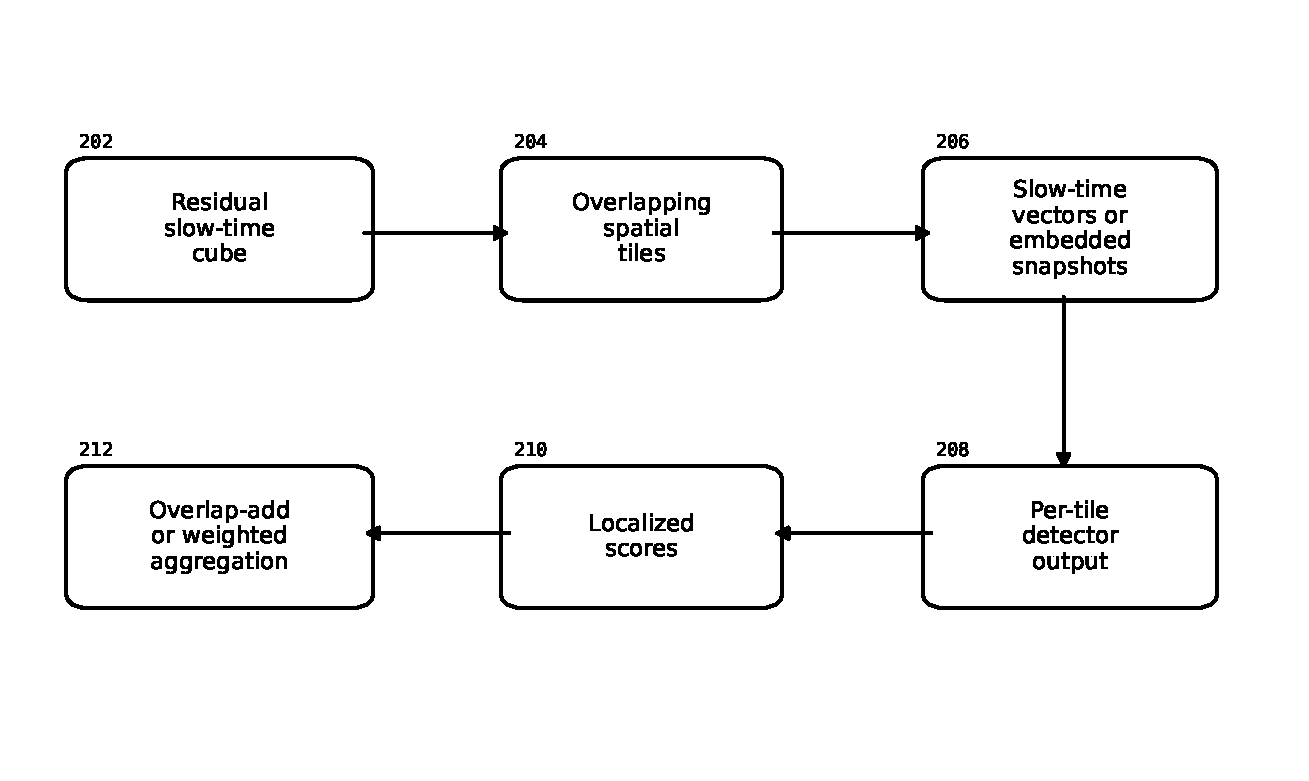
\includegraphics[width=\textwidth,height=0.72\textheight,keepaspectratio]{figs/figure_02_local_processing.pdf}
\caption*{Figure 2. Localized spatial support extraction, temporal support formation, per-support detector scoring, and aggregation back into a score map.}
\end{figure}
\clearpage

\begin{figure}[p]
\centering
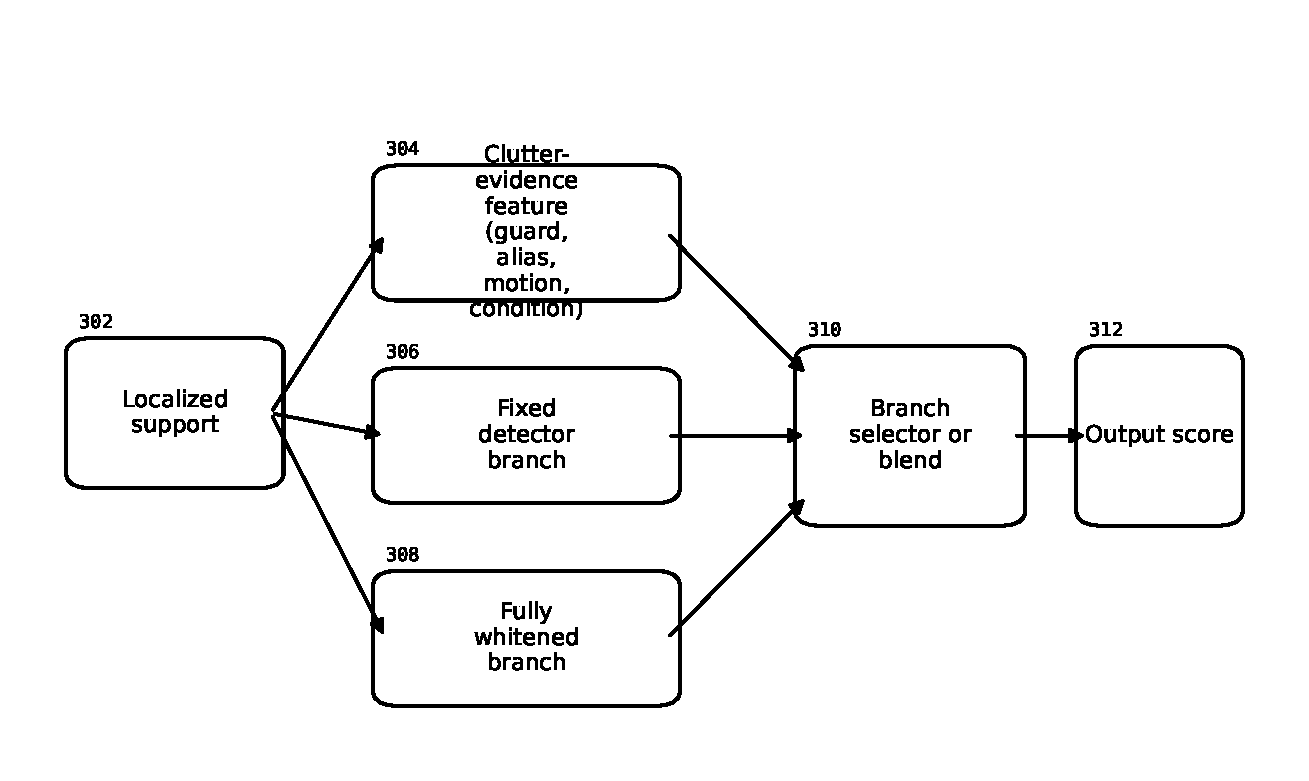
\includegraphics[width=\textwidth,height=0.72\textheight,keepaspectratio]{figs/figure_03_adaptive_switch.pdf}
\caption*{Figure 3. Adaptive branch selection using clutter-evidence features to choose between a fixed detector branch and a fully whitened detector branch.}
\end{figure}
\clearpage

\begin{figure}[p]
\centering
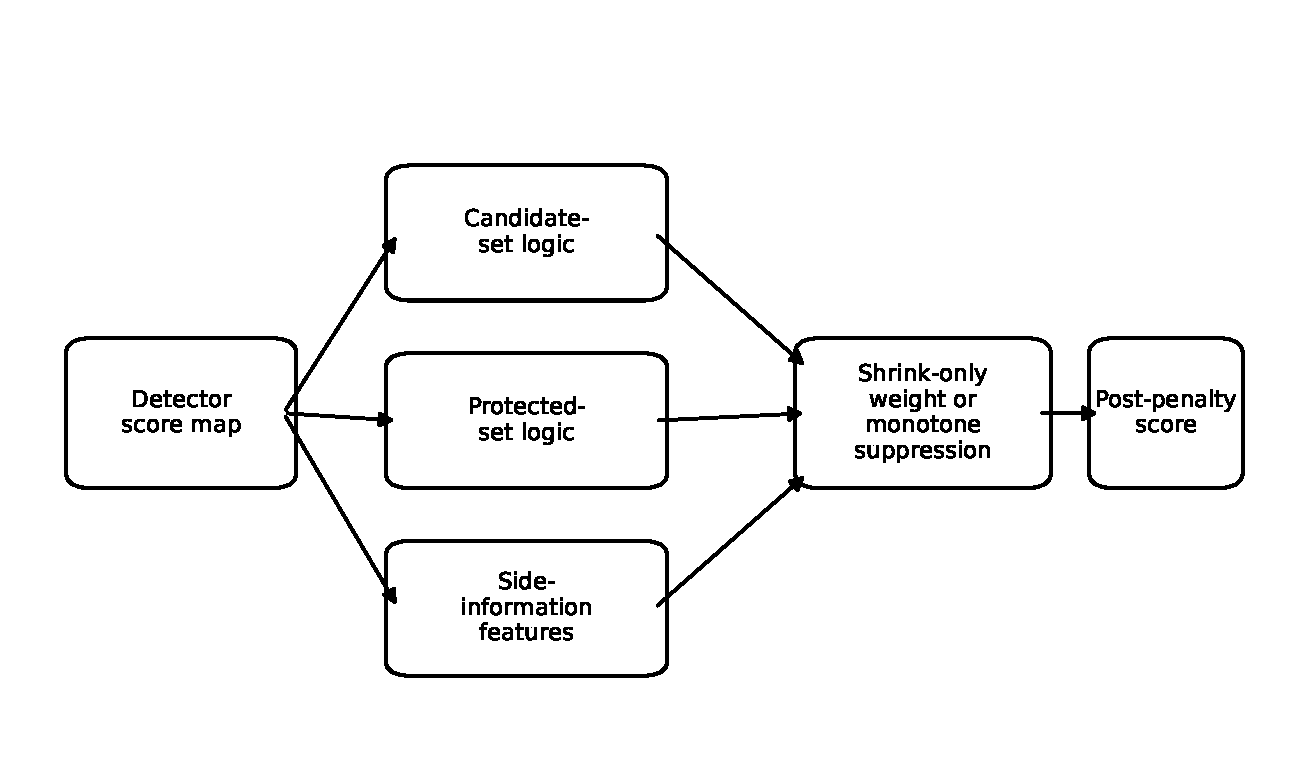
\includegraphics[width=\textwidth,height=0.72\textheight,keepaspectratio]{figs/figure_04_penalty_layer.pdf}
\caption*{Figure 4. Optional shrink-only penalty layer with candidate-set logic, protected-set logic, and post-penalty score generation.}
\end{figure}
\clearpage

\begin{figure}[p]
\centering
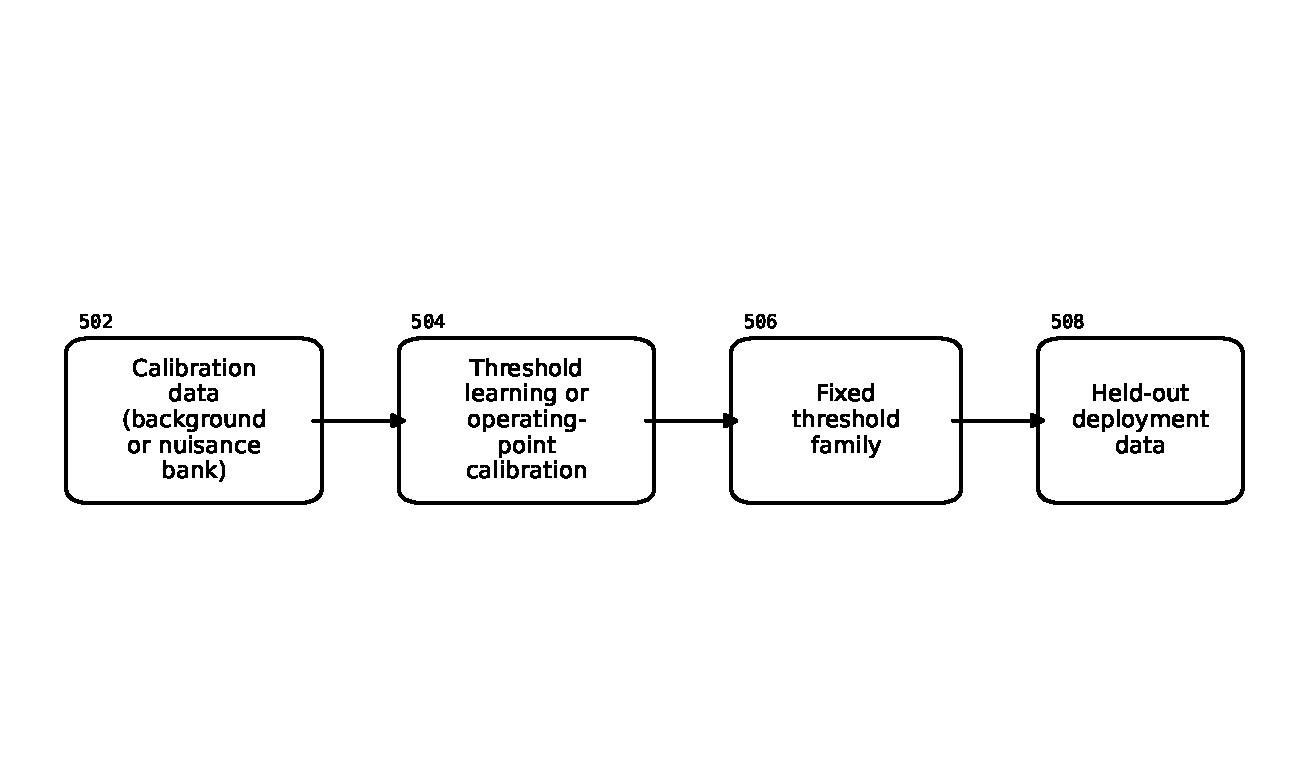
\includegraphics[width=\textwidth,height=0.72\textheight,keepaspectratio]{figs/figure_05_threshold_transfer.pdf}
\caption*{Figure 5. Threshold calibration and transfer workflow in which thresholds are learned from calibration data and applied to held-out deployment data without per-window retuning.}
\end{figure}
\clearpage

\begin{figure}[p]
\centering
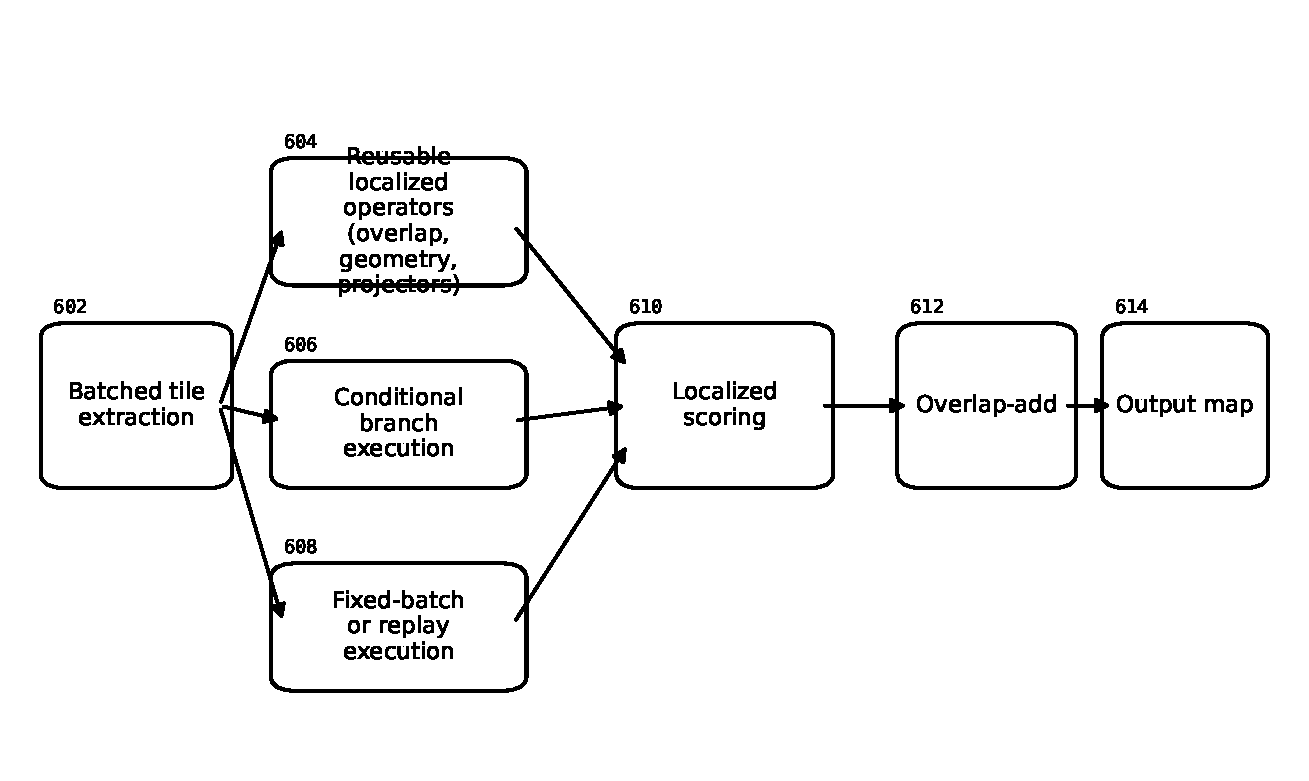
\includegraphics[width=\textwidth,height=0.72\textheight,keepaspectratio]{figs/figure_06_realtime_architecture.pdf}
\caption*{Figure 6. Exact-output-preserving real-time execution architecture using reusable localized operators, conditional branch execution, and batched score generation.}
\end{figure}
\clearpage

\end{document}
